\section{Metodología}
\label{sec:methodology}

\subsection{Flujo general}

El desarrollo siguió un flujo iterativo: definición del contexto y clases,
preparación del dataset, construcción de la aplicación web, integración del proxy
de predicción, entrenamiento del modelo en Custom Vision y validación del producto.
Antes de clasificar la roca, la API aplica un detector binario roca/no-roca para
rechazar imágenes fuera de dominio. El siguiente diagrama resume el flujo de interacción en la aplicación.

\begin{mermaid}[style=editorial, width=0.95\linewidth, pos=H, caption={Flujo general de predicción en Litoteca}]
  sequenceDiagram
    autonumber
    actor U as Usuario
    participant W as Litoteca Web
    participant F as CF Pages Function
    participant CV as Custom Vision
    participant WK as Wiki cache (build)

    U->>W: Captura o carga imagen
    W->>W: Preprocesa y valida imagen
    W->>F: POST /api/predict
    F->>CV: Solicita detección roca/no-roca
    CV-->>F: Probabilidades rock / not rock
    alt No es roca o rock < 0.5
      F-->>W: 422 no es roca
      W-->>U: Muestra mensaje: no se identificó roca
    else Es roca
      F->>CV: Solicita clasificación por clase
      CV-->>F: Predicciones por clase
      F-->>W: JSON normalizado (top, confianza, margen)
      W->>WK: Consulta extracto cacheado
      WK-->>W: Extracto y fuente CC BY-SA
      W-->>U: Muestra ficha, confianza, gemelas y contexto
    end
\end{mermaid}

\subsection{Selección y preparación del dataset}

\subsubsection{Fuente}

Se utilizó el dataset \emph{Rock Classification} de Kaggle, exportado originalmente
desde Roboflow~\cite{rockdataset}. El export contenía 4.212 imágenes en 9 clases,
con aumentos sintéticos generados por Roboflow (3 versiones por imagen original:
espejo, recorte, brillo/exposición, entre otros).

La copia local del dataset se mantuvo en \texttt{data/raw/rock-data} y el resultado
preparado en \texttt{data/prepared}. Por tamaño, \texttt{data/} no se versiona en
Git; su reconstrucción se documenta con \texttt{tools/prepare\_dataset.py}.

\subsubsection{Problemas encontrados}

El análisis inicial detectó dos problemas importantes:

\begin{itemize}
  \item \textbf{Fuga entre splits}: el mismo original aparecía en train y valid/test
        con distintos aumentos. Se encontraron 89 originales compartidos entre train
        y valid, 43 entre train y test, y 15 entre valid y test.
  \item \textbf{Conflictos de etiqueta}: 22 pares de imágenes casi idénticas tenían
        etiquetas distintas, especialmente entre clases síliceas como chert,
        diatomite y geiserita.
\end{itemize}

\subsubsection{Limpieza y reconstrucción}

El script \texttt{tools/prepare\_dataset.py} realizó:

\begin{enumerate}
  \item Agrupación por imagen original (cluster), no por archivo aumentado.
  \item Cálculo de hash perceptual \texttt{dHash} para detectar duplicados y
        casi-duplicados~\cite{zauner2010implementation}.
  \item Reconstrucción de splits sin intersección de clusters: 85/15 estratificado
        para train/valid sobre originales no reservados a test.
  \item En valid/test se conservó un representante por cluster (medoid).
  \item En train se conservaron aumentos del export original.
  \item Generación de manifiestos: \texttt{manifest.csv}, \texttt{stats.json},
        \texttt{conflicts.csv}, \texttt{near\_duplicates.csv}, \texttt{descartadas.csv}.
\end{enumerate}

\begin{table}[H]
  \centering
  \caption{Dataset preparado inicial (con aumentos en train)}
  \label{tab:dataset-prepared}
  \begin{tabular}{@{}lrrrr@{}}
    \toprule
    Clase & Originales & Train & Valid & Test \\
    \midrule
    Basalto & 198 & 398 & 27 & 15 \\
    Basalto olivínico & 192 & 359 & 18 & 19 \\
    Arcilla & 198 & 410 & 26 & 12 \\
    Conglomerado & 200 & 414 & 23 & 13 \\
    Lutita & 195 & 367 & 26 & 20 \\
    Diatomita & 198 & 383 & 22 & 19 \\
    Sílex & 195 & 379 & 21 & 14 \\
    Geiserita & 181 & 354 & 21 & 11 \\
    Yeso & 197 & 364 & 25 & 23 \\
    \midrule
    \textbf{Total} & \textbf{1754} & \textbf{3428} & \textbf{209} & \textbf{146} \\
    \bottomrule
  \end{tabular}
\end{table}

\subsubsection{Versión limpia para Custom Vision}

Para el entrenamiento en Custom Vision se generó \texttt{data/prepared-clean-train}
con la política: una imagen por cluster en todos los splits, excluyendo clusters
involucrados en conflictos de etiqueta. Los casi-duplicados entre clusters se
marcaron en reporte, pero no se eliminaron automáticamente para evitar una limpieza
demasiado agresiva sin revisión visual.

\begin{table}[H]
  \centering
  \caption{Dataset limpio usado para entrenamiento}
  \label{tab:dataset-clean}
  \begin{tabular}{@{}lrrr@{}}
    \toprule
    Clase & Train & Valid & Test \\
    \midrule
    Basalto & 156 & 27 & 15 \\
    Sílex & 148 & 21 & 14 \\
    Arcilla & 152 & 26 & 12 \\
    Conglomerado & 155 & 23 & 13 \\
    Diatomita & 145 & 22 & 19 \\
    Yeso & 144 & 25 & 23 \\
    Basalto olivínico & 143 & 18 & 19 \\
    Lutita & 145 & 26 & 20 \\
    Geiserita & 137 & 21 & 11 \\
    \midrule
    \textbf{Total} & \textbf{1325} & \textbf{209} & \textbf{146} \\
    \bottomrule
  \end{tabular}
\end{table}

Esta versión reduce redundancia sintética y evita que el modelo aprenda artefactos
de aumentos del export. Custom Vision puede aplicar sus propias transformaciones de
entrenamiento; por eso se prefirió subir imágenes limpias.

\subsection{Entrenamiento y modelos}

\subsubsection{Clasificador multiclase}

El entrenamiento se realizó en Azure Custom Vision con un proyecto multiclase de
Litoteca~\cite{azurecustomvision}. La Figura~\ref{fig:custom-vision} muestra la
captura de los proyectos usados en el espacio de trabajo.

\begin{figure}[H]
  \centering
  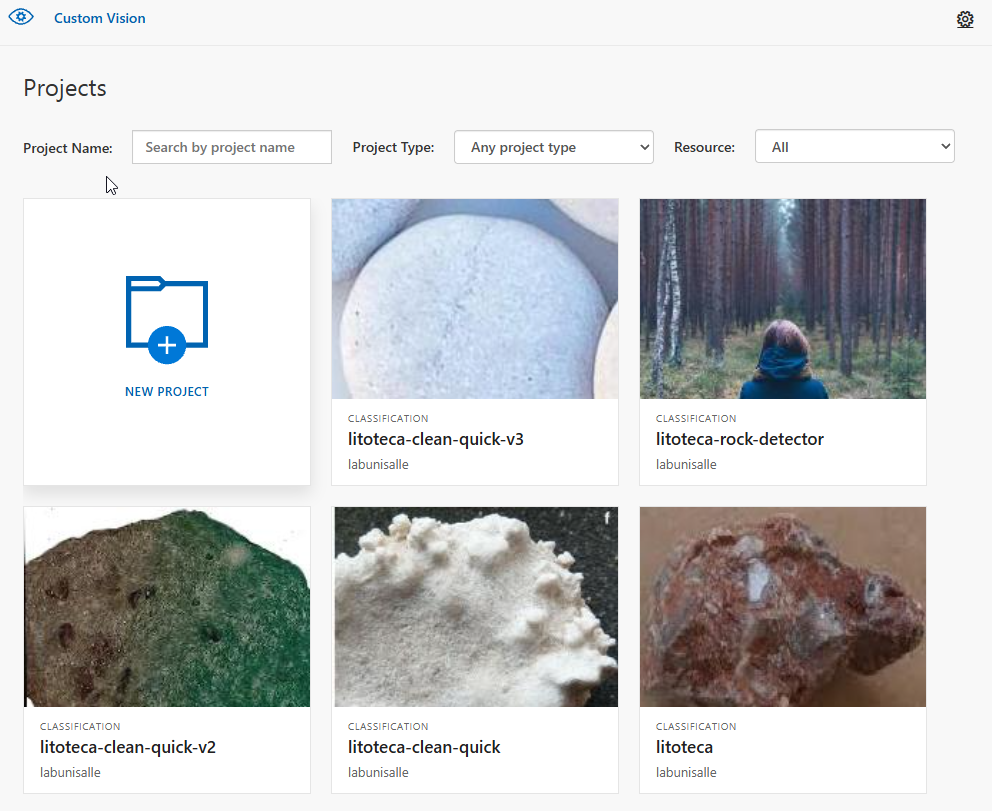
\includegraphics[width=0.95\linewidth]{assets/images/custom-vision-projects.png}
  \caption{Proyectos de Litoteca en Azure Custom Vision, incluyendo las iteraciones Quick y el detector roca/no-roca.}
  \label{fig:custom-vision}
\end{figure}

Se trabajaron tres iteraciones Quick completadas sobre el dataset limpio y una
iteración Advanced que terminó siendo la de mejor desempeño:

\begin{itemize}
  \item \textbf{Quick v1} (proyecto \texttt{litoteca-clean-quick}, iteración
        \texttt{6276ca2b-ad3e-4ca4-93ea-3be210b98771}): primera iteración
        completada, con validación API de 95/146 aciertos (65.07\%).
  \item \textbf{Quick v2} (proyecto \texttt{litoteca-clean-quick-v2}, iteración
        \texttt{4792fd31-2f7a-4505-9c72-71c1c3ffe4b8}): entrenamiento completado,
        publicado como \texttt{litoteca-v1} en \texttt{labunisalle-Prediction};
        luego fue reemplazado por la iteración Advanced publicada como
        \texttt{litoteca-v2}.
\end{itemize}

\begin{table}[H]
  \centering
  \caption{Comparación global entre iteraciones Quick completadas}
  \label{tab:metricas-globales}
  \begin{tabular}{@{}lrrr@{}}
    \toprule
    Iteración & Precision & Recall & AP \\
    \midrule
    Quick v1 (6276ca2b) & 83.08\% & 52.43\% & 72.74\% \\
    Quick v2 (4792fd31) & 84.88\% & 54.48\% & 77.77\% \\
    Quick v3 (9354cec6) & 79.70\% & 54.58\% & 74.64\% \\
    Advanced (d538f641) & 98.66\% & 96.22\% & 98.42\% \\
    \bottomrule
  \end{tabular}
\end{table}

La iteración Advanced mejora las métricas globales respecto a todas las Quick,
especialmente en recall y AP. El desempeño es alto y parejo en las nueve clases,
incluidas las que concentraban confusión en las iteraciones anteriores
(\emph{shale}, \emph{clay} y \emph{chert}).

\subsubsection{Quick v3 y decisión de cierre}

Se entrenó Quick v3 como iteración curada adicional (proyecto
\texttt{litoteca-clean-quick-v3}, \texttt{601da1f6-4fa9-47c0-9177-26284667cc56},
iteración \texttt{9354cec6-b49a-400e-9ce9-0c4230254fd9}, tipo \texttt{Quick}).
El dataset de entrenamiento partió de v2 y recuperó 131 imágenes de v1 en clases
débiles/confusas (\emph{chert}, \emph{clay}, \emph{conglomerate},
\emph{diatomite}, \emph{shale}, \emph{siliceous-sinter}), quedando en 1278 train,
193 valid y 144 test.

Quick v3 obtuvo P 79.70\%, R 54.58\% y AP 74.64\%, con validación sintética API
de 96/146 (65.75\%). Al no superar a Quick v2 (P 84.88\%, R 54.48\%, AP 77.77\%;
101/146, 69.18\%), no se promovió.

\subsubsection{Iteración Advanced y modelo final}

La iteración Advanced del proyecto \texttt{litoteca}
(\texttt{d15445ca-24b1-4bcc-aa80-244fb2b8fd6a}, iteración
\texttt{d538f641-63da-4db3-8827-fe2e1f91cee9}) terminó después de 410 minutos de
entrenamiento y superó ampliamente a las iteraciones Quick: P 98.66\%, R 96.22\% y
AP 98.42\%. En la validación sintética API obtuvo 109/146 (74.66\%), frente a
101/146 (69.18\%) de Quick v2. Por ese resultado se publicó como
\texttt{litoteca-v2} en \texttt{labunisalle-Prediction} y se conectó a la aplicación
como modelo final, manteniendo el mismo contrato de la API.

\begin{table}[H]
  \centering
  \caption{Métricas por clase de la iteración Advanced}
  \label{tab:metricas-clase}
  \begin{tabular}{@{}lrrr@{}}
    \toprule
    Clase & Precision & Recall & AP \\
    \midrule
    basalt & 97.53\% & 98.75\% & 98.72\% \\
    chert & 98.61\% & 93.42\% & 97.15\% \\
    clay & 100.00\% & 91.46\% & 96.78\% \\
    conglomerate & 100.00\% & 97.59\% & 98.87\% \\
    diatomite & 97.40\% & 97.40\% & 97.69\% \\
    gypsum & 98.59\% & 95.89\% & 99.89\% \\
    olivine-basalt & 100.00\% & 98.61\% & 100.00\% \\
    shale & 97.30\% & 97.30\% & 98.72\% \\
    siliceous-sinter & 98.55\% & 95.77\% & 98.51\% \\
    \bottomrule
  \end{tabular}
\end{table}

\subsubsection{Detector roca/no-roca}

Para reducir falsos positivos ante imágenes fuera de dominio, se entrenó un modelo
binario separado en Custom Vision con dos etiquetas: \texttt{rock} y
\texttt{not\_rock}. El dataset de detección (\texttt{data/rock-detector}) contiene
150 imágenes de roca y 150 imágenes no-roca. La iteración
\texttt{2d92f618-115e-4a73-a9ed-006002782c7c} del proyecto
\texttt{2dc1aedb-f66c-4fb1-abc5-54c253440052} se publicó como
\texttt{litoteca-detector-v1} en \texttt{labunisalle-Prediction}.

\begin{table}[H]
  \centering
  \caption{Métricas del detector roca/no-roca}
  \label{tab:detector-metricas}
  \begin{tabular}{@{}lrrr@{}}
    \toprule
    Etiqueta / Global & Precision & Recall & AP \\
    \midrule
    not\_rock & 100.00\% & 100.00\% & --- \\
    rock & 100.00\% & 96.70\% & --- \\
    \midrule
    \textbf{Global} & \textbf{100.00\%} & \textbf{98.28\%} & \textbf{99.97\%} \\
    \bottomrule
  \end{tabular}
\end{table}

La Function \texttt{functions/api/predict.js} consulta primero el detector. Si la
etiqueta superior es \texttt{not\_rock} o la probabilidad de \texttt{rock} es menor
que 0.5, la API responde con HTTP 422 y código \texttt{no\_es\_roca}; solo cuando la
imagen pasa este guardrail se invoca el clasificador multiclase. Las credenciales y
endpoints de predicción se manejan como variables de entorno en Cloudflare Pages,
incluidos \texttt{CUSTOM\_VISION\_DETECTOR\_PROJECT} y
\texttt{CUSTOM\_VISION\_DETECTOR\_ITERATION}.

\subsection{Desarrollo de la aplicación}

\subsubsection{Arquitectura}

La aplicación es un sitio estático sin build: HTML, CSS y JavaScript vanilla. La
predicción se consume mediante una Cloudflare Pages Function en
\texttt{functions/api/predict.js}, que valida la imagen, ejecuta primero el detector
roca/no-roca y, solo si la imagen pasa el guardrail, envía la solicitud al
clasificador multiclase de Custom Vision. La respuesta se normaliza al contrato de
Litoteca.

\begin{table}[H]
  \centering
  \caption{Componentes principales de la aplicación}
  \label{tab:componentes}
  \begin{tabular}{@{}p{3.8cm}p{8.6cm}@{}}
    \toprule
    Componente & Responsabilidad \\
    \midrule
    \texttt{index.html} & Estructura de vistas: inicio, cámara, resultado e historial. \\
    \texttt{assets/app.js} & Lógica de UI, cámara, subida, historial local y presentación de resultados. \\
    \texttt{assets/app.css} & Sistema visual editorial/papel. \\
    \texttt{assets/fichas.js} & Fichas curadas de las 9 clases. \\
    \texttt{assets/wiki.js} & Extractos cacheados de Wikipedia con atribución CC BY-SA. \\
    \texttt{functions/api/predict.js} & Proxy a Custom Vision, guardrail roca/no-roca, validación y contrato. \\
    \texttt{sw.js} & Service worker para caché de recursos estáticos y comportamiento sin conexión~\cite{w3cserviceworkers}. \\
    \texttt{scripts/gates.sh} & Gates deterministas, pruebas de contrato y smoke test de navegador. \\
    \bottomrule
  \end{tabular}
\end{table}

\subsubsection{Interfaz de usuario}

La interfaz se diseñó con enfoque móvil, accesible y educativo. Incluye:

\begin{itemize}
  \item Captura con cámara o carga de imagen.
  \item Vista de resultado con clase, confianza, margen y alternativas.
  \item Fichas con explicación: qué es, cómo se formó, gemelas y señales.
  \item Historial local en el navegador.
  \item Modo sin conexión para recursos ya cacheados; la predicción en línea se
        desactiva cuando no hay red.
\end{itemize}

\subsubsection{Generación de ilustraciones}

Para reforzar el valor pedagógico, se generaron ilustraciones del proceso geológico
de cada roca. Las ilustraciones se produjeron con \texttt{facet + ComfyUI}
(workflow \texttt{flux2-klein-4b}) a partir de una pieza reproducible
(\texttt{tools/procesos-geologicos.toml}). Luego se optimizaron a WebP/PNG y se les
agregaron etiquetas de texto manualmente, evitando texto sintético generado por el
modelo de imagen.

\begin{figure}[H]
  \centering
  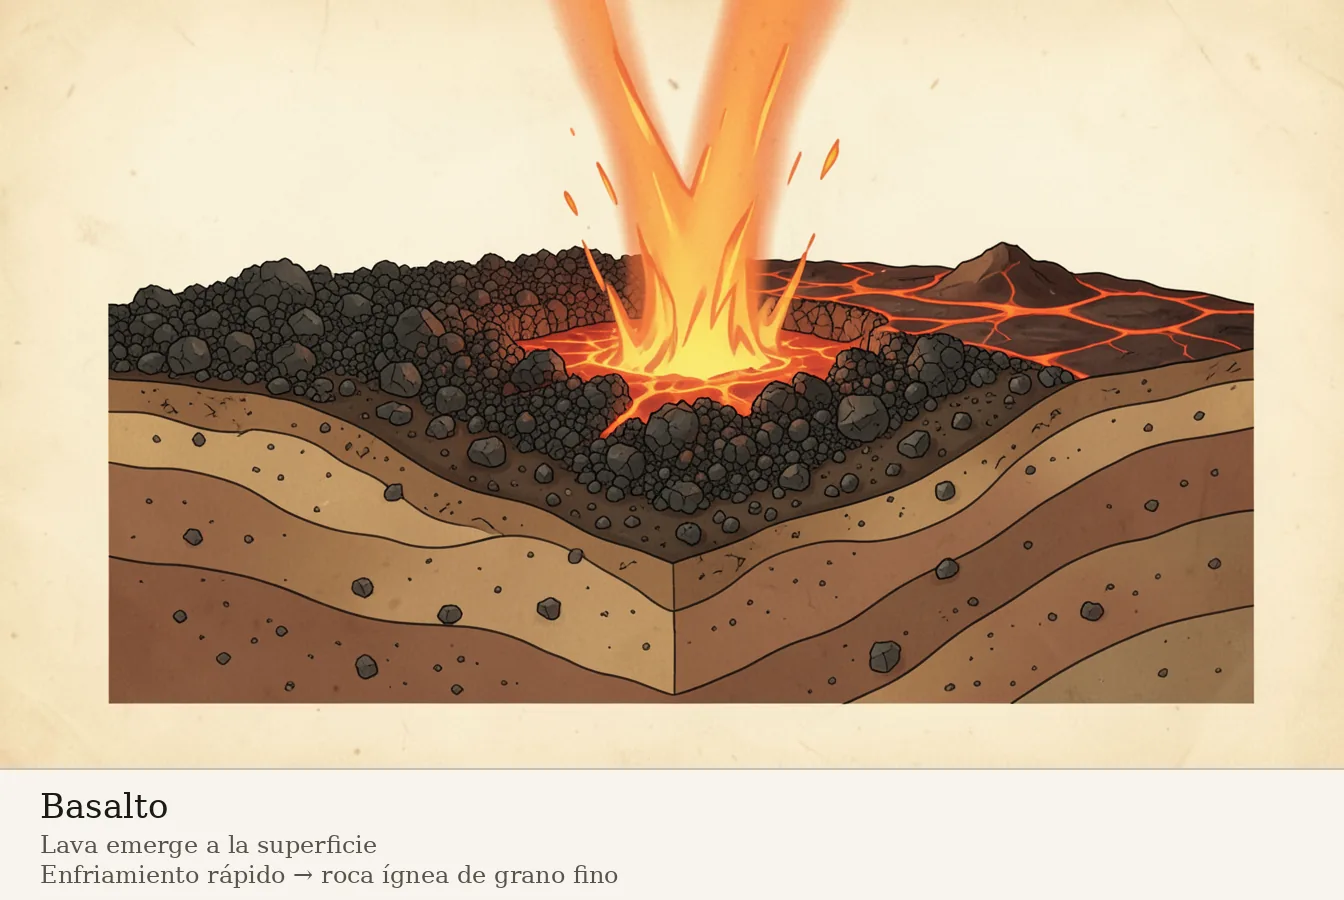
\includegraphics[width=0.82\linewidth]{assets/images/basalt.png}
  \caption{Ejemplo de ilustración generada para el proceso de formación del basalto}
  \label{fig:basalt}
\end{figure}

\subsection{Despliegue}

La aplicación se despliega en Cloudflare Pages~\cite{cloudflarepages}. El flujo de
despliegue usa GitHub Actions con \texttt{workflow\_dispatch} desde la rama
\texttt{develop}, entorno \texttt{production}, y \texttt{wrangler pages deploy}.
Los secretos de Cloudflare se configuran en GitHub Environment secrets; los secretos
de Custom Vision, incluidos los del detector roca/no-roca, se configuran en
Cloudflare Pages como variables de runtime de la Function.

La versión pública está disponible en \url{https://litoteca.pages.dev/}
\cite{litotecaapp}. La demo en video está disponible en
\url{https://youtu.be/X435kZhNOG8}.
